\hypertarget{shapefunctionRBF_8h}{
\section{src/shapefunctionRBF.h File Reference}
\label{shapefunctionRBF_8h}\index{src/shapefunctionRBF.h@{src/shapefunctionRBF.h}}
}
Function for interpolation of basic variables by means of Radial basis Functions. 

{\tt \#include \char`\"{}shapefunction.h\char`\"{}}\par


Include dependency graph for shapefunctionRBF.h:\nopagebreak
\begin{figure}[H]
\begin{center}
\leavevmode
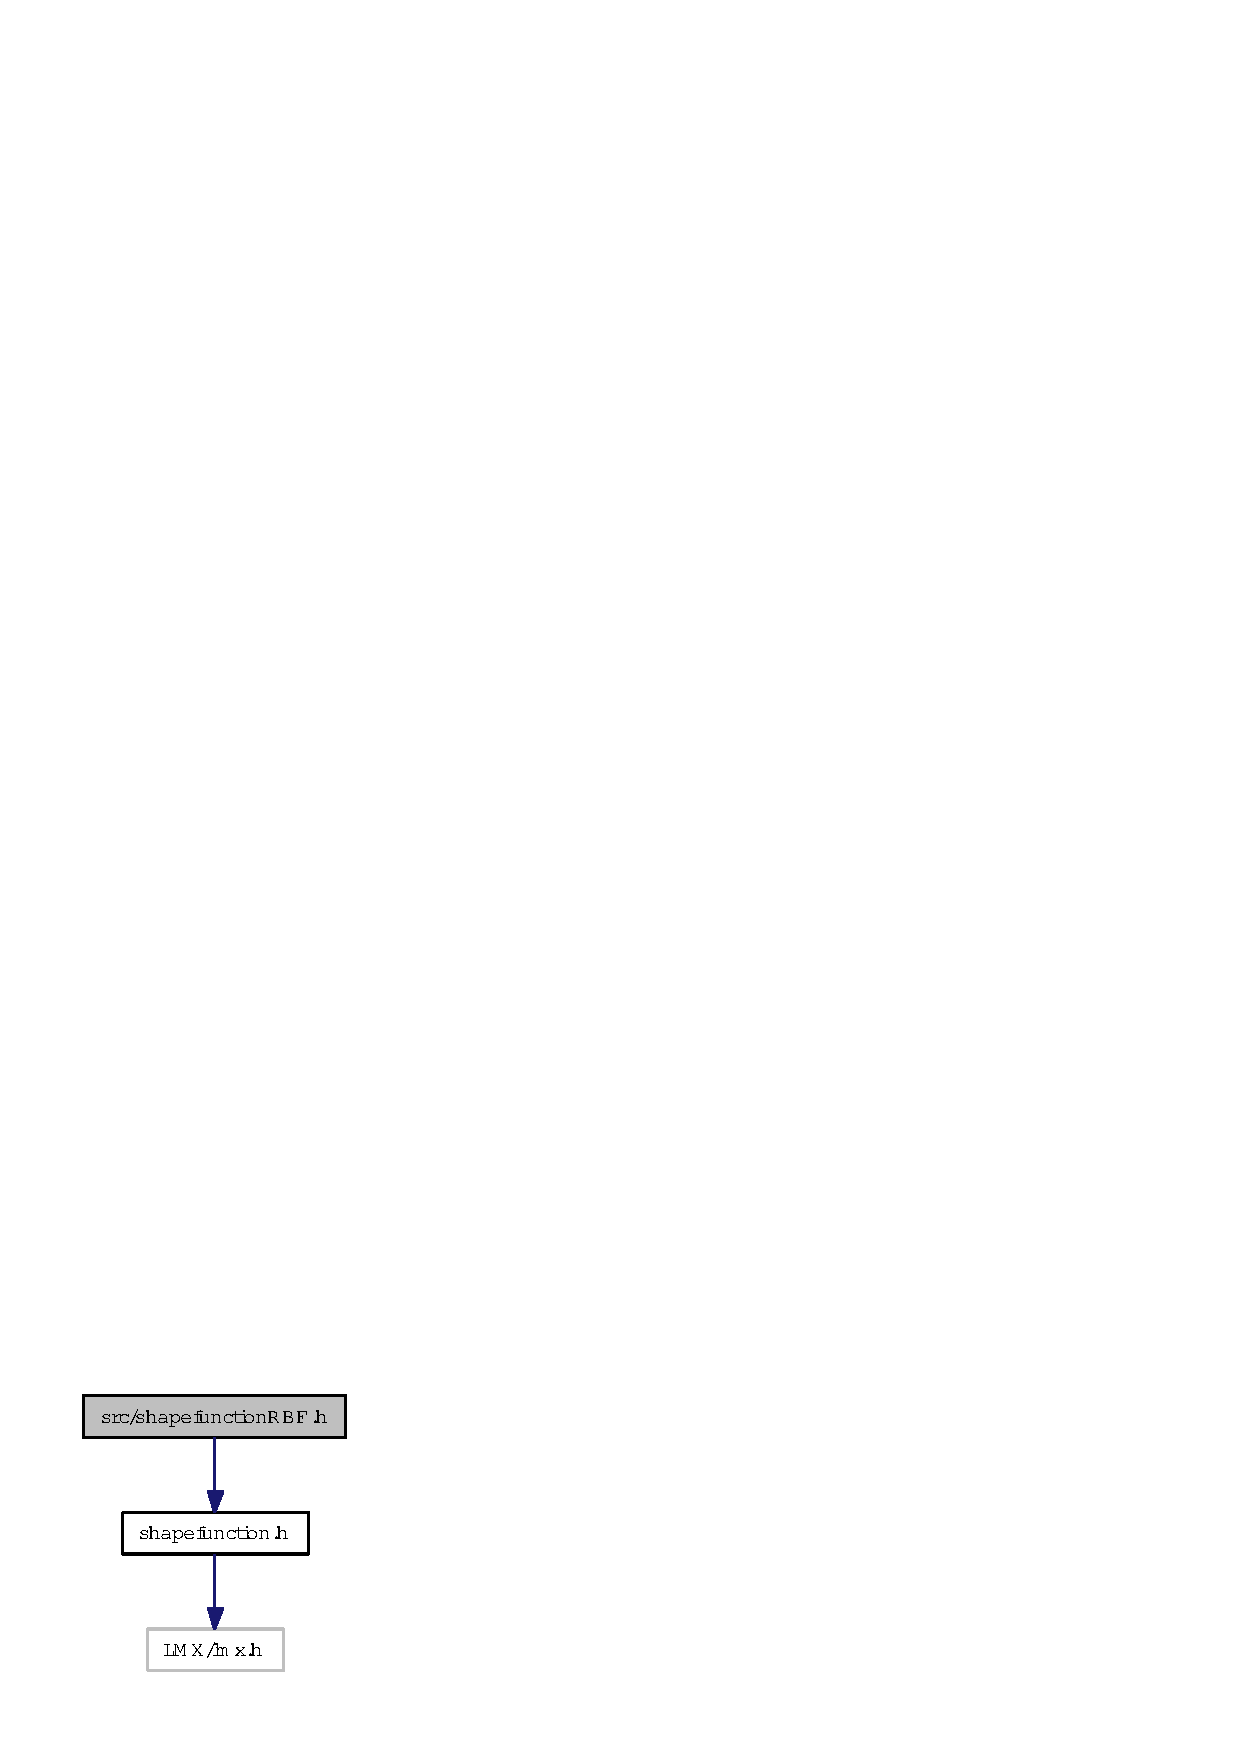
\includegraphics[width=85pt]{shapefunctionRBF_8h__incl}
\end{center}
\end{figure}


This graph shows which files directly or indirectly include this file:\nopagebreak
\begin{figure}[H]
\begin{center}
\leavevmode
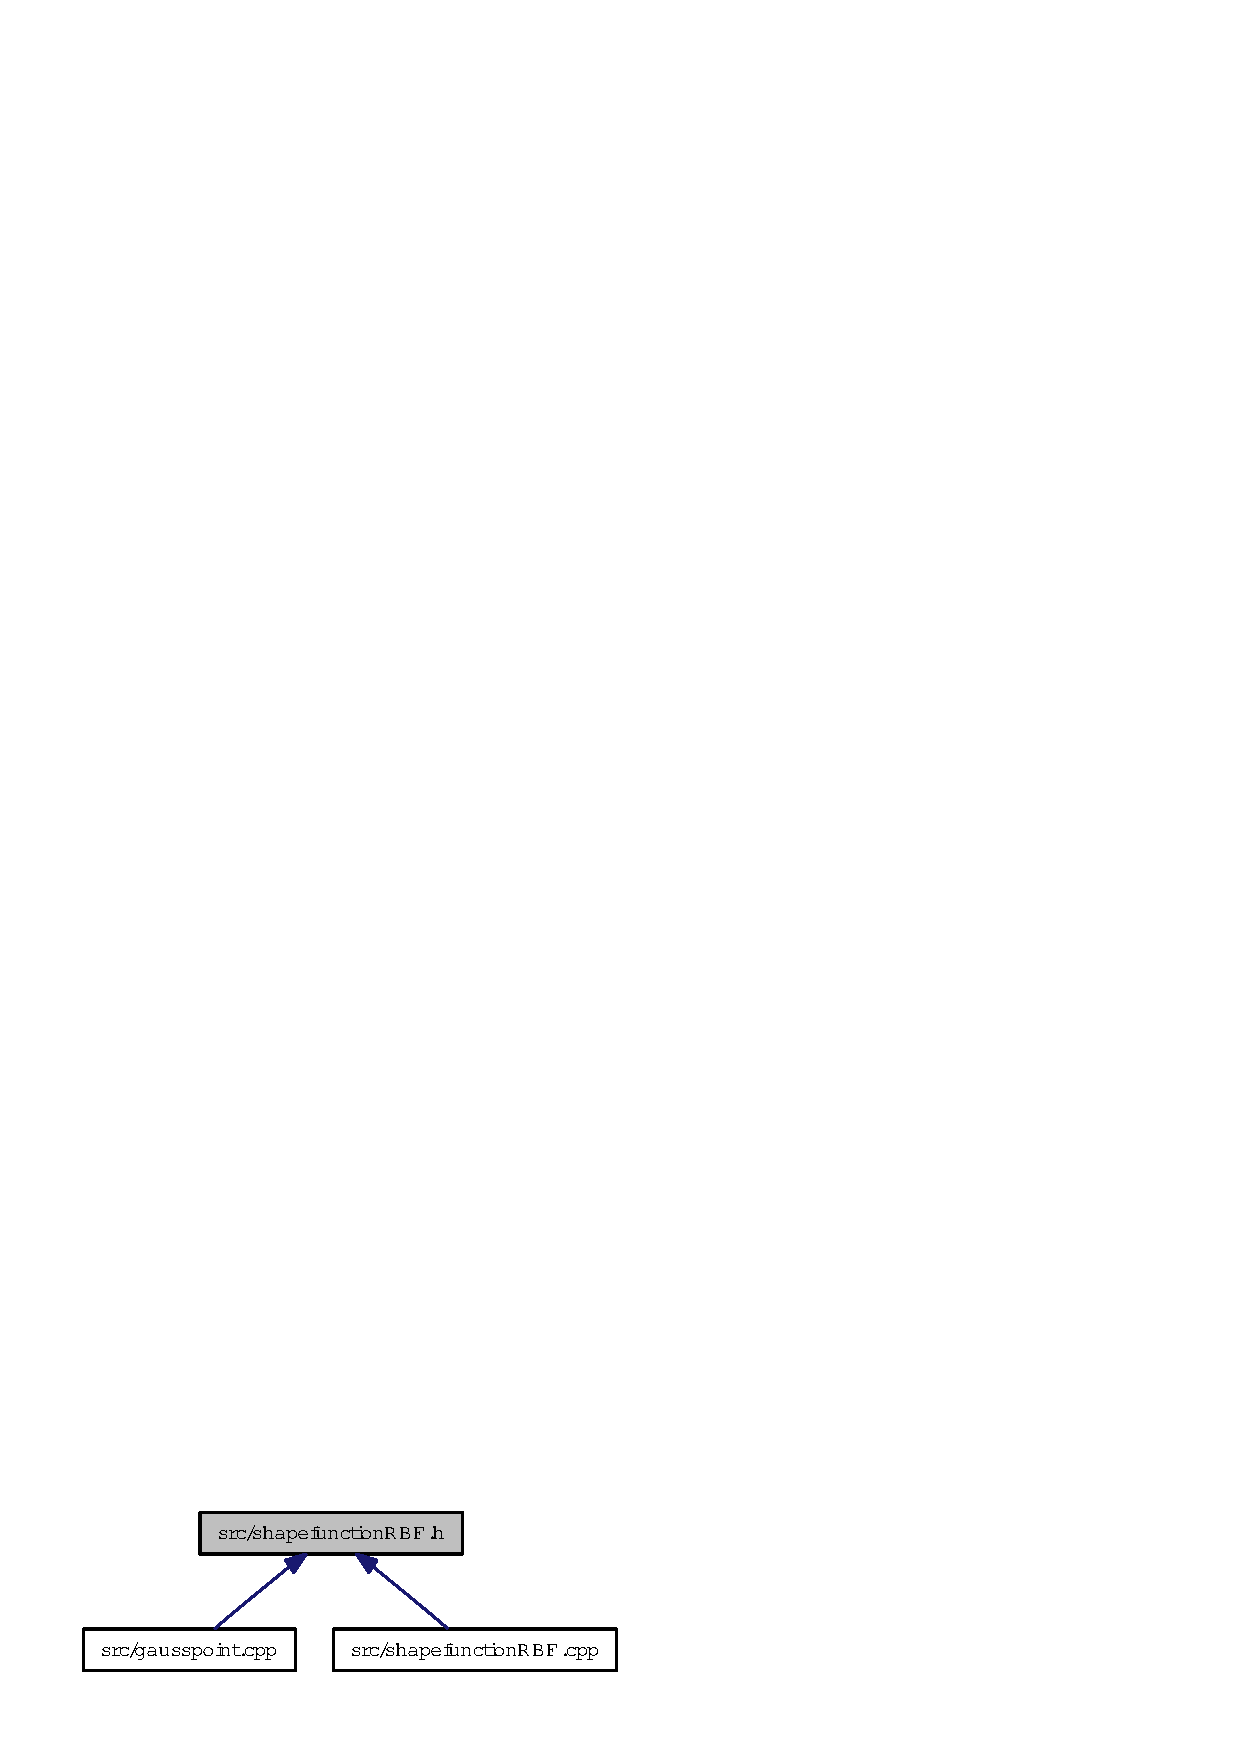
\includegraphics[width=150pt]{shapefunctionRBF_8h__dep__incl}
\end{center}
\end{figure}
\subsection*{Namespaces}
\begin{CompactItemize}
\item 
namespace \hyperlink{namespacemknix}{mknix}
\end{CompactItemize}
\subsection*{Classes}
\begin{CompactItemize}
\item 
class \hyperlink{classmknix_1_1ShapeFunctionRBF}{mknix::ShapeFunctionRBF}
\end{CompactItemize}


\subsection{Detailed Description}
Function for interpolation of basic variables by means of Radial basis Functions. 

\begin{Desc}
\item[Author:]Daniel Iglesias Ibáñez \end{Desc}


Definition in file \hyperlink{shapefunctionRBF_8h-source}{shapefunctionRBF.h}.